% This tex file is available under a
% Creative Commons Attribution-Share Alike license (CC BY-SA 2.0).
% http://creativecommons.org/licenses/by-sa/2.0/
% Copyright © 2013 Rodrigo Hausen
\documentclass{beamer}
\usepackage[utf8]{inputenc}
\usepackage{lmodern}
\usepackage[T1]{fontenc}
\usepackage[portuguese,brazil]{babel}
\usepackage{url}
\usepackage{listings}
\usepackage{color}
\usepackage{textcomp}
\usepackage{pdfpages}
\usepackage{fancyvrb}
\usepackage{enumerate}
\usepackage{alltt}
\usepackage{array}
\usepackage{slashbox}
%\usepackage[pdf]{pstricks}
%\usepackage{auto-pst-pdf}
%\usepackage{icomma} % para vírgula decimal / decimal comma
\definecolor{listinggray}{gray}{0.9}
\definecolor{mediumgray}{rgb}{0.6,0.6,0.6}
\definecolor{lbcolor}{rgb}{0.9,0.9,0.9}
\lstset{
    backgroundcolor=\color{lbcolor},
    tabsize=4,
    rulecolor=,
    basicstyle=\scriptsize,
    upquote=true,
    aboveskip={1.5\baselineskip},
    columns=fixed,
    showstringspaces=false,
    extendedchars=true,
    breaklines=true,
    prebreak = \raisebox{0ex}[0ex][0ex]{\ensuremath{\hookleftarrow}},
    frame=single,
    showtabs=false,
    showspaces=false,
    showstringspaces=false,
    identifierstyle=\ttfamily,
    keywordstyle=\color[rgb]{0,0,1},
    commentstyle=\color[rgb]{0.133,0.545,0.133},
    stringstyle=\color[rgb]{0.627,0.126,0.941},
}
\definecolor{pinegreen}{RGB}{0,139,114}
\definecolor{pgr}{RGB}{0,139,114}

\definecolor{aquamarine}{RGB}{0,181,190}
\definecolor{aqm}{RGB}{0,181,190}

\definecolor{skyblue}{RGB}{100,227,251}
\definecolor{skb}{RGB}{100,227,251}

\definecolor{pnk}{RGB}{255,150,150}

\newcommand{\comment}[1]{{\color{structure.fg!70!white}\footnotesize #1}}

\newcommand{\WD}[1]{\fbox{#1}\hspace{-0.5pt}}
\newcommand{\FWD}[1]{%
\fbox{%
\vbox to 10pt{\vfil%
\hbox to 0.8cm{\hfill#1\hfill}%
\vfil}%
}\hspace{-0.5pt}%
}

\def\A{\texttt{A}}
\def\B{\texttt{B}}
\def\C{\texttt{C}}
\def\D{\texttt{D}}
\def\E{\texttt{E}}
\def\F{\texttt{F}}

\usetheme{Boadilla}
%\usetheme{umbc2}
\usefonttheme{structuresmallcapsserif}
\usecolortheme{seahorse}

\title{Aula 14: Aplicações de Flip-flops}
\subtitle{Circuitos Digitais}
\author{Rodrigo Hausen}
\institute{CMCC -- UFABC} 
\date{15 de março de 2013}

\newcommand{\Not}[1]{\overline{#1}}
\def\And{\,}

\begin{document}

\begin{frame}
\maketitle

\vspace{-1cm}

\begin{center}
\url{http://compscinet.org/circuitos}
\end{center}

\end{frame}

%%%%%%%%%%%%%%%%%%%%%%%%%%%%%%%%%%%%%%%%%%%%%%%%%
\begin{frame}
\frametitle{Relembrando: Flip-flop S-R}

\textbf{Flip-flop S-R sensível à borda de descida do clock} (borda negativa)

\begin{center}
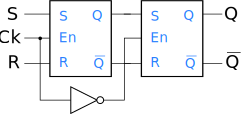
\includegraphics{images/flipflopRS_circuit}
\hspace{2ex}
\raisebox{50pt}{\Huge$=$}
\hspace{2ex}
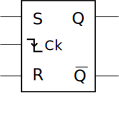
\includegraphics{images/flipflopRS_blackbox}

\vspace{12pt}

\begin{tabular}{ccc||cl}
$S$ & $R$ &        $Ck$       & $Q_i$ \\
\cline{1-4}
 0  &  0  &        $?$        & $Q_{i-1}$  & (mantem $Q$) \\
 0  &  1  &  1$\rightarrow$0  &     0      & (reset $Q$) \\
 1  &  0  &  1$\rightarrow$0  &     1      & (set $Q$) \\
 1  &  1  &  1$\rightarrow$0  &     X  & (proibido) \\
\end{tabular}
\end{center}

\end{frame}

%%%%%%%%%%%%%%%%%%%%%%%%%%%%%%%%%%%%%%%%%%%%%%%%%
\begin{frame}
\frametitle{Relembrando: Flip-flop S-R}

\textbf{Flip-flop S-R sensível à borda de subida do clock} (borda positiva)

\begin{center}
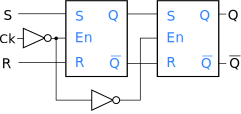
\includegraphics{images/flipflopRSpos_circuit}
\hspace{2ex}
\raisebox{50pt}{\Huge$=$}
\hspace{2ex}
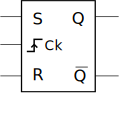
\includegraphics{images/flipflopRSpos_blackbox}

\vspace{12pt}

\begin{tabular}{ccc||cl}
$S$ & $R$ &        $Ck$       & $Q_i$ \\
\cline{1-4}
 0  &  0  &        $?$        & $Q_{i-1}$  & (mantem $Q$) \\
 0  &  1  &  0$\rightarrow$1  &     0      & (reset $Q$) \\
 1  &  0  &  0$\rightarrow$1  &     1      & (set $Q$) \\
 1  &  1  &  0$\rightarrow$1  &     X  & (proibido) \\
\end{tabular}
\end{center}

\end{frame}

%%%%%%%%%%%%%%%%%%%%%%%%%%%%%%%%%%%%%%%%%%%%%%%%%
\begin{frame}
\frametitle{Relembrando: Flip-flop D}

Flip-flop D sensível à borda de descida.

\begin{center}
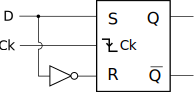
\includegraphics{images/flipflopD_circuit}%
\hspace{3ex}%
\raisebox{40pt}{\Huge$=$}%
\hspace{3ex}%
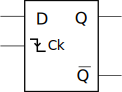
\includegraphics{images/flipflopD_blackbox}

\vspace{12pt}

\begin{tabular}{cc||cl}
 $D$ &        $Ck$       & $Q_i$ \\
\cline{1-3}
  0  &  1$\rightarrow$0  &     0      & (reset = armazena 0) \\
  1  &  1$\rightarrow$0  &     1      & (set = armazena 1) \\
\end{tabular}
\end{center}

\end{frame}

%%%%%%%%%%%%%%%%%%%%%%%%%%%%%%%%%%%%%%%%%%%%%%%%%
\begin{frame}
\frametitle{Relembrando: Flip-flop J-K}

\begin{center}
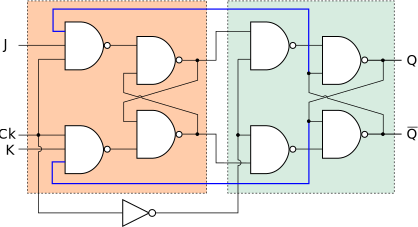
\includegraphics[width=0.5\textwidth]{images/flipflopJK2}%
\hspace{3ex}%
\raisebox{40pt}{\Huge$=$}%
\hspace{3ex}%
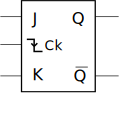
\includegraphics{images/flipflopJK_blackbox}

\vspace{12pt}


\begin{tabular}{ccc||ccl}
$J$ & $K$ &        $Ck$       & $Q_i$           & $\Not{Q_i}$ \\[4pt]
\cline{1-5}
    &     &                   &                 &    \\[-8pt]
 0  &  0  &        $?$        & $Q_{i-1}$       & $\Not{Q_{i-1}}$ & (mantem) \\
 0  &  1  &  0$\rightarrow$1  &     0           &       1         & (kill = reset) \\
 1  &  0  &  0$\rightarrow$1  &     1           &       0         & (jump = set) \\ 
 1  &  1  &  0$\rightarrow$1  & $\Not{Q_{i-1}}$ & $Q_{i-1}$       & (inverte) \\
\end{tabular}

\end{center}

\end{frame}

%%%%%%%%%%%%%%%%%%%%%%%%%%%%%%%%%%%%%%%%%%%%%%%%%
\begin{frame}
\frametitle{Flip-flops: Aplicações}

Contador de $3$ bits:

\vspace{12pt}

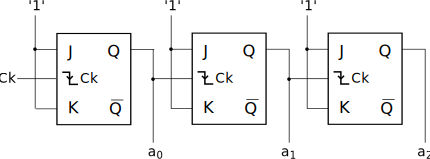
\includegraphics[width=\textwidth]{images/counter}

\end{frame}

%%%%%%%%%%%%%%%%%%%%%%%%%%%%%%%%%%%%%%%%%%%%%%%%%
\begin{frame}
\frametitle{Flip-flops: Aplicações}

\textbf{Problema:} Faça um contador de $0$ até $5$.

\pause

\vspace{12pt}

Estados de $a_2, a_1, a_0$, respectivamente:\\
\texttt{000}, \texttt{001}, \texttt{010},
\texttt{011}, \texttt{100}, \texttt{101},
\texttt{000}, \ldots

\pause

\vspace{12pt}

Como fazer com que todas as saídas $Q$ dos flip-flops
J-K tornem-se $0$ antes da transição
\texttt{111}$\rightarrow$\texttt{000}
dos estados das saídas?

\pause

\vspace{12pt}

Precisamos alterar o flip-flop J-K para que possamos
zerar $Q$ independentemente de detectarmos uma borda
do clock. Para isso, precisamos voltar ao latch S-R
com enable.

\end{frame}

%%%%%%%%%%%%%%%%%%%%%%%%%%%%%%%%%%%%%%%%%%%%%%%%%
\begin{frame}
\frametitle{Latch S-R com Enable, Preset e Clear}

Problema: latch S-R só responde às entradas
$S$ e $R$ quando $En = 1$. Queremos poder fazer
\emph{reset} e \emph{set}, independentemente do
estado de $En$.

\begin{center}
\only<1>{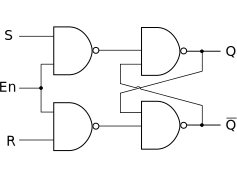
\includegraphics{images/latchRSnandEnable_circuit}}%
\only<2>{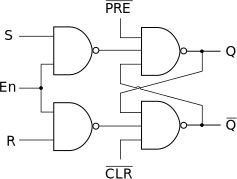
\includegraphics{images/latchRSnandEnablepreclr_circuit}}
\end{center}

\pause

Solução: adicione duas entradas ativas em nível baixo,
$\Not{PRE}$ e $\Not{CLR}$, às portas NAND das saídas.

\end{frame}

%%%%%%%%%%%%%%%%%%%%%%%%%%%%%%%%%%%%%%%%%%%%%%%%%
\begin{frame}
\frametitle{Latch S-R com Enable, Preset e Clear}

Comportamento do Latch S-R com Enable, Preset e Clear:
\begin{itemize}
\uncover<2->{
\item quando $\Not{PRE} = 1$ e $\Not{CLR} = 1$, idêntico ao latch S-R com enable;
}
\uncover<3->{
\item quando $\Not{PRE} = 1$ e $\Not{CLR} = 0$, ocorre \emph{reset} ($Q = 0$);
}
\uncover<4->{
\item quando $\Not{PRE} = 0$ e $\Not{CLR} = 1$, ocorre \emph{set} ($Q = 1$);
}
\uncover<5->{
\item é proibido $\Not{PRE} = 0$ e $\Not{CLR} = 0$
}
\end{itemize}

\begin{center}
\only<1,5->{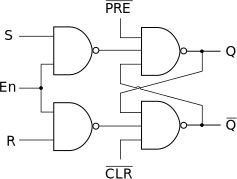
\includegraphics{images/latchRSnandEnablepreclr_circuit}}%
\only<2>{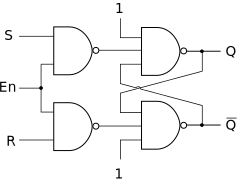
\includegraphics{images/latchRSnandEnablepreclr11_circuit}}%
\only<3>{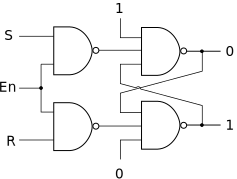
\includegraphics{images/latchRSnandEnablepreclr10_circuit}}%
\only<4>{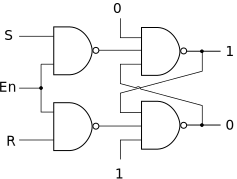
\includegraphics{images/latchRSnandEnablepreclr01_circuit}}%
\hspace{2ex}%
\uncover<6->{\raisebox{68pt}{\Huge=}}%
\hspace{2ex}%
\uncover<7->{%
\raisebox{10pt}{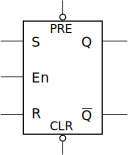
\includegraphics{images/latchRSEnablePreClr_blackbox}}%
}
\end{center}

\end{frame}

%%%%%%%%%%%%%%%%%%%%%%%%%%%%%%%%%%%%%%%%%%%%%%%%%
\begin{frame}
\frametitle{Entradas assíncronas: Preset e Clear}

Usando latches S-R com Enable, Preset e Clear, é possível fazer
flip-flops S-R, D e J-K com entradas Preset e Clear ativas em nível baixo.

\begin{itemize}
\item As entradas $\Not{PRE}$ e $\Not{CLR}$ são ditas
\textbf{assíncronas} pois elas interferem no funcionamento
dos flip-flops \textbf{independentemente do \emph{clock}}
(ao contrário das demais entradas, que só afetam o flip-flop
em uma das bordas do clock)
\end{itemize}

\hspace{2ex}
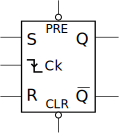
\includegraphics{images/flipflopRSPreClr_blackbox}
\hfill
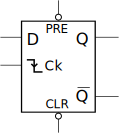
\includegraphics{images/flipflopDPreClr_blackbox}
\hfill
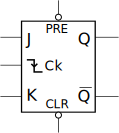
\includegraphics{images/flipflopJKPreClr_blackbox}
\hspace{2ex}

\end{frame}

%%%%%%%%%%%%%%%%%%%%%%%%%%%%%%%%%%%%%%%%%%%%%%%%%
\begin{frame}
\frametitle{Voltando ao contador}

Voltando ao problema original: fazer um contador de $0$ até $5$.

\vspace{12pt}

Contador de $3$ bits (conta de $0$ a $7$):

\vspace{6pt}

\texttt{000} $\rightarrow$ \texttt{001} $\rightarrow$ \texttt{010}
$\rightarrow$ \texttt{011} $\rightarrow$ \texttt{100} 
$\rightarrow$ \texttt{101} $\rightarrow$ \texttt{110} 
$\rightarrow$ \texttt{111}\\
\begin{picture}(263,12)
\put(8,0){\vector(0,1){10}}
\put(8,0){\line(1,0){250}}
\put(258,0){\line(0,1){10}}
\end{picture}

\vspace{12pt}

\pause

Como evitar a transição \texttt{101} $\rightarrow$ \texttt{110},
transformando-a em \texttt{101} $\rightarrow$ \texttt{000}?

\vspace{6pt}

\texttt{000} $\rightarrow$ \texttt{001} $\rightarrow$ \texttt{010}
$\rightarrow$ \texttt{011} $\rightarrow$ \texttt{100} 
$\rightarrow$ \texttt{101} {\color{gray} $\rightarrow$ \texttt{110} 
$\rightarrow$ \texttt{111}}\\
\begin{picture}(263,12)
\put(8,0){\vector(0,1){10}}
\put(8,0){\line(1,0){180}}
\put(188,0){\line(0,1){10}}
\end{picture}

\vspace{12pt}

\pause

Idéia: fazer reset dos flip-flops do contador assim que
a contagem for excedida!

\vspace{6pt}

\pause

Isto acontece quando chegamos em $5 + 1 = (110)_2$

\end{frame}

%%%%%%%%%%%%%%%%%%%%%%%%%%%%%%%%%%%%%%%%%%%%%%%%%
\begin{frame}
\frametitle{Voltando ao contador}

Agora, o problema é detectar, por meio de um sinal
ativo de \textbf{nível baixo}, quando $(a_2 a_1 a_0)_2 = (110)_2$

\pause

\vspace{12pt}

Detecção por nível alto: $a_2 \, a_1 \, \Not{a_0}$

\pause

\vspace{6pt}

Detecção por nível baixo: $\Not{a_2 \, a_1 \, \Not{a_0}}$

\pause

\vspace{6pt}

\only<1-4>{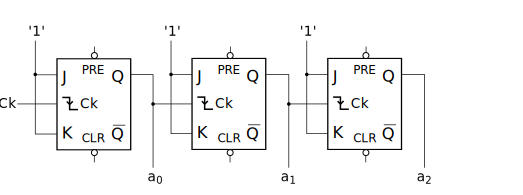
\includegraphics[width=\textwidth]{images/counter_modulo6_0}}%
\only<5>{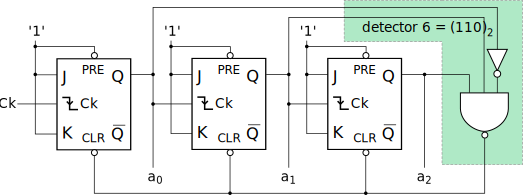
\includegraphics[width=\textwidth]{images/counter_modulo6}}%

\end{frame}

%%%%%%%%%%%%%%%%%%%%%%%%%%%%%%%%%%%%%%%%%%%%%%%%%
\begin{frame}
\frametitle{Contador módulo $m$}

{\small
\begin{itemize}
\item \textbf{Contador módulo $m$}: circuito digital com uma
entrada de clock que conta de $0$ até $m-1$.
\end{itemize}

Exemplo: contador módulo $6$, que conta de $0$ a $5$.\\[12pt]
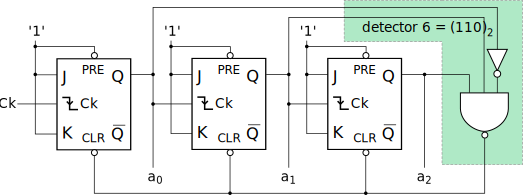
\includegraphics[width=\textwidth]{images/counter_modulo6}

}
\end{frame}

%%%%%%%%%%%%%%%%%%%%%%%%%%%%%%%%%%%%%%%%%%%%%%%%%
\begin{frame}
\frametitle{Flip-flops: Aplicações}

Faça o diagrama de forma de onda para o circuito abaixo
e diga o que ele faz.

\vspace{12pt}

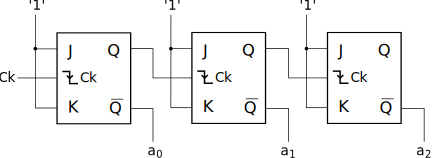
\includegraphics[width=\textwidth]{images/downcounter}

(Solução na lousa) \pause É um contador regressivo para
$3$ bits: \texttt{111}, \texttt{110}, \texttt{101},
\ldots, \texttt{001}, \texttt{000}, \texttt{111}, \ldots

\end{frame}

%%%%%%%%%%%%%%%%%%%%%%%%%%%%%%%%%%%%%%%%%%%%%%%%%
\begin{frame}
\frametitle{Flip-flops: Aplicações}

Faça o diagrama de forma de onda para o circuito abaixo
e diga o que ele faz (entrada: $Ck$, saída: $Q$)

\begin{center}
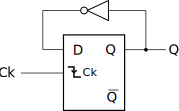
\includegraphics{images/flipflopT}
\end{center}


(Solução na lousa) \pause Funciona como um flip-flop J-K
com as entradas J = 1 e K = 1, ou seja, inverte a saída
a cada borda de descida do clock.

\end{frame}

%%%%%%%%%%%%%%%%%%%%%%%%%%%%%%%%%%%%%%%%%%%%%%%%%
\begin{frame}
\frametitle{Flip-flops: Aplicações}

Faça o diagrama de forma de onda para o circuito abaixo
e diga o que ele faz (entrada: $Ck$, saídas: $a_2, a_1, a_0$)

\begin{center}
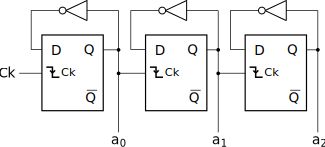
\includegraphics{images/flipflopTcounter}
\end{center}

(Solução na lousa) \pause Outra maneira de implementar
um contador de $3$ bits.

\end{frame}


%%%%%%%%%%%%%%%%%%%%%%%%%%%%%%%%%%%%%%%%%%%%%%%%%
\begin{frame}
\frametitle{Flip-flops: Aplicações}

\begin{itemize}
\item \textbf{Registrador síncrono:} só atualiza o
dado na borda de descida do clock. Possui uma entrada $\Not{CLR}$,
ativa em nível baixo.\\[6pt]

\hspace{6ex}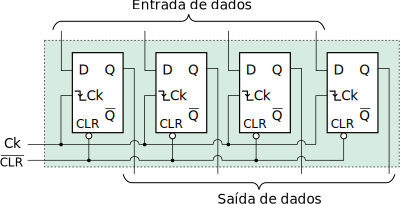
\includegraphics[scale=0.7]{images/sync_register}\pause\\[6pt]
\hspace*{\fill}\raisebox{24pt}{\Huge=}\hspace{6ex}\pause
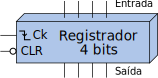
\includegraphics[scale=0.9]{images/sync_register_blackbox}\hspace{3ex}

\end{itemize}

\end{frame}

%%%%%%%%%%%%%%%%%%%%%%%%%%%%%%%%%%%%%%%%%%%%%%%%%
\begin{frame}
\frametitle{Flip-flops: Aplicações}

\begin{itemize}
\item O que faz o circuito abaixo? (Entrada: $Ck$, Saídas: $a_3, a_2, a_1, a_0$)
\end{itemize}

\begin{minipage}{0.6\textwidth}
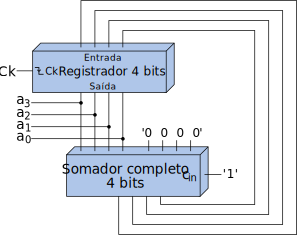
\includegraphics[scale=0.95]{images/sync_counter}
\end{minipage}
\hfill\pause%
\begin{minipage}{0.3\textwidth}
Contador de $4$ bits\\[12pt]

\pause

Diferentemente dos anteriores,
este contador é
\textbf{síncrono}:\\
todas
as saídas são sincronizadas
\end{minipage}

\end{frame}

%%%%%%%%%%%%%%%%%%%%%%%%%%%%%%%%%%%%%%%%%%%%%%%%%
\begin{frame}
\frametitle{Projeto de contadores síncronos}

Modelo geral de um contador síncrono:\\[12pt]

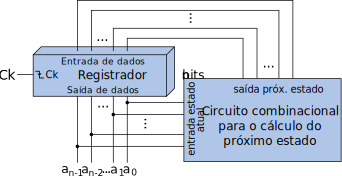
\includegraphics{images/sync_counter_general}

\end{frame}

%%%%%%%%%%%%%%%%%%%%%%%%%%%%%%%%%%%%%%%%%%%%%%%%%
\begin{frame}
\frametitle{Projeto de contadores síncronos}

\textbf{Exemplo:} projetar um contador de código Gray.\\[12pt]

\textbf{Passo Zero:} Fazer o diagrama de estados.
\begin{center}
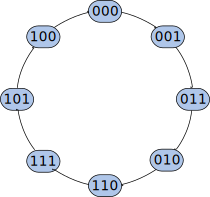
\includegraphics[scale=0.9]{images/gray_counter_states}
\end{center}
Cada transição é feita em uma borda de subida do clock.

\end{frame}

%%%%%%%%%%%%%%%%%%%%%%%%%%%%%%%%%%%%%%%%%%%%%%%%%
\begin{frame}
\frametitle{Projeto de contadores síncronos}

\textbf{Passo Um:} Obter e simplificar as expressões para cada uma
das saídas do circuito combinacional para o próximo estado.\\[12pt]

\begin{minipage}{0.47\textwidth}
\begin{tabular}{|ccc||ccc|}
\hline
\multicolumn{3}{|c||}{atual} &
\multicolumn{3}{c|}{próximo} \\
$a_2$ & $a_1$ & $a_0$        & $A_2$ & $A_1$ & $A_0$ \\
\hline
  0   &   0   &   0   \pause &   0   &   0   &   1   \\ \pause
  0   &   0   &   1   \pause &   0   &   1   &   1   \\ \pause
  0   &   1   &   1   \pause &   0   &   1   &   0   \\ \pause
  0   &   1   &   0          &   1   &   1   &   0   \\ \pause
  1   &   1   &   0          &   1   &   1   &   1   \\ \pause
  1   &   1   &   1          &   1   &   0   &   1   \\ \pause
  1   &   0   &   1          &   1   &   0   &   0   \\ \pause
  1   &   0   &   0          &   0   &   0   &   0   \\
\hline
\end{tabular}
\end{minipage}
\hfill
\pause
\begin{minipage}{0.5\textwidth}
\textbf{Para casa:} faça o mapa de Karnaugh para cada saída.
Você obterá:\\

$A_0 = \Not{a_1} \, \Not{a_2} + a_1 \, a_2 \pause = \Not{a_1 \oplus a_2}$\\

\pause

$A_1 = a_0 \, \Not{a_2} + \Not{a_0} \, a_1$\\

\pause

$A_2 = \Not{a_0} \, a_1 + a_0 \, a_2$
\end{minipage}

\end{frame}

%%%%%%%%%%%%%%%%%%%%%%%%%%%%%%%%%%%%%%%%%%%%%%%%%
\begin{frame}
\frametitle{Projeto de contadores síncronos}

\textbf{Passo Dois:} Diagrama \only<5->{completo} do circuito.
\only<2>{$A_0 = \Not{a_1 \oplus a_2}$}%
\only<3>{$A_1 = a_0 \, \Not{a_2} + \Not{a_0} \, a_1$}%
\only<4>{$A_2 = \Not{a_0} \, a_1 + a_0 \, a_2$}

\vspace{12pt}

\hspace{8ex}%
\only<1>{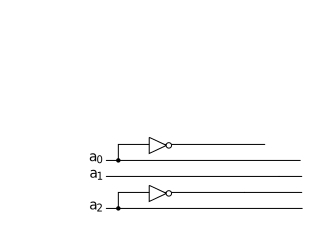
\includegraphics{images/gray_counter_circuit3}}%
\only<2>{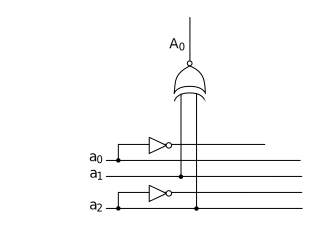
\includegraphics{images/gray_counter_circuit2}}%
\only<3>{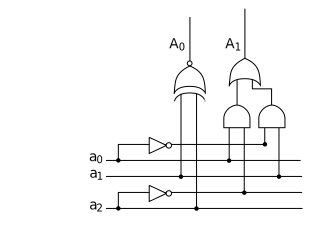
\includegraphics{images/gray_counter_circuit1}}%
\only<4>{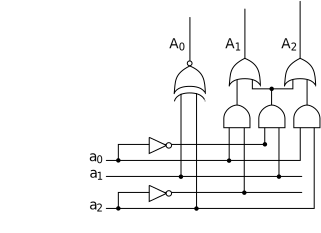
\includegraphics{images/gray_counter_circuit0}}%
\only<5->{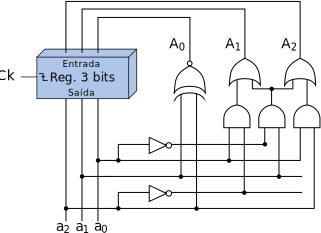
\includegraphics{images/gray_counter_circuit}}%

\end{frame}

%%%%%%%%%%%%%%%%%%%%%%%%%%%%%%%%%%%%%%%%%%%%%%%%%
\begin{frame}
\frametitle{Para casa}

\begin{itemize}
\item Leia as seções 7-3 e 8-1 do livro do Floyd
\item Exercícios do capítulo 7: autoteste 9, problemas 14, 15, 16, 17, 18, 25 e 26.
\item Exercícios do capítulo 8: autotestes 1, 3 até 7, problemas 1 a 3.
\item Leia o texto ``Projeto de Máquinas de Estado'' no site
\item Resolva os problemas 14 a 19 do capítulo 8.
\begin{itemize}
\item Nos problemas 16 a 19, use registradores síncronos\\
(ignore a parte da questão onde é dito ``use flip-flops J-K'')
\end{itemize}
\end{itemize}

\end{frame}

%%%%%%%%%%%%%%%%%%%%%%%%%%%%%%%%%%%%%%%%%%%%%%%%%
\begin{frame}
\frametitle{Exercícios adicionais}

{\small

\textbf{1.} Como fazer um contador com flip-flops J-K sensíveis
à borda de \textbf{subida}?\\[6pt]

\pause

\textbf{2.} Usando flip-flops J-K, faça o circuito de um
\textbf{contador de década} (também chamado contador decádico, é
um contador módulo 10)\\[6pt]

\pause

\textbf{3.} Usando flip-flops J-K, faça um contador decádico
regressivo:\\
\texttt{1001}, \texttt{1000}, \texttt{0111}, \ldots, \texttt{0001},
\texttt{0000}, \texttt{1001}, \ldots\\[6pt]

\pause

\textbf{4.} Usando flip-flops D sensíveis à borda de \textbf{descida},
faça um registrador síncrono para palavras de $4$ bits,
sensível à borda de \textbf{subida}. Entradas: $Ck$, $\Not{CLR}$ e
$WE$ (write enable = habilita escrita).\\[6pt]

\pause

Em cada exercício abaixo, assuma que os únicos componentes disponíveis
são um registrador de $4$ bits e um somador completo de $4$ bits.\\[6pt]

\textbf{5.} Faça um contador progressivo para $4$ bits com passo $2$:
\texttt{0000}, \texttt{0010}, \texttt{0100}, \texttt{0110}, \ldots
Entradas: $Ck$ (clock) e $\Not{CLR}$ (zera o contador).\\[6pt]

\pause

\textbf{6.} Faça um contador progressivo/regressivo (up/down) para $4$
bits com três entradas: $Ck$ (clock), $\Not{CLR}$ (zera o contador) e
$\Not{U}/D$ (se $0$ = progressivo; se $1$ = regressivo).

}

\end{frame}

\end{document}
